\documentclass[a4paper,twoside,12pt,fleqn]{scrartcl}
\usepackage[margin=2.5cm]{geometry}
%\usepackage{fancyref}
%\usepackage{graphicx}
%\usepackage{float}
%\usepackage{tabularx}
%\usepackage{booktabs,array}
%\usepackage{caption}
\usepackage{subcaption}
\usepackage{amsmath}
\usepackage{amsthm}
\usepackage{amssymb}
\usepackage{mathtools} % for multlined enviornment
%\usepackage{amsfonts}
%\usepackage{enumitem}
\usepackage[hyphens]{url}
\geometry{a4paper}
\usepackage{amssymb}%---allows \mathbb{R/Z/etc.} (numbers sets)
\usepackage{scrextend} %for eddmargin environment
\usepackage{caption}
\usepackage{titlesec}


%%%%[for python code] %%%%%%
\usepackage{listings}
\usepackage{color}

\definecolor{dkgreen}{rgb}{0,0.6,0}
\definecolor{gray}{rgb}{0.5,0.5,0.5}
\definecolor{mauve}{rgb}{0.58,0,0.82}

\lstset{frame=tb,
  language=Python,
  aboveskip=3mm,
  belowskip=3mm,
  showstringspaces=false,
  columns=flexible,
  basicstyle={\small\ttfamily},
  numbers=none,
  numberstyle=\tiny\color{gray},
  keywordstyle=\color{blue},
  commentstyle=\color{dkgreen},
  stringstyle=\color{mauve},
  breaklines=true,
  breakatwhitespace=true,
  tabsize=3
}

%\titlelabel{\thetitle\quad}


\renewcommand{\vec}[1]{\mathbf{#1}}
\newcommand{\parder}[2]{\frac{\partial{#1}}{\partial{#2}}}

\newcommand{\sectionbreak}{\clearpage}

\newcommand{\lagrangian}[1]{\mathcal{L}(\vec{#1})}
\newcommand{\vecprod}[2]{\vec{#1}^T{\vec{#2}}}
\newcommand{\expwx}{\exp(\vecprod{w}{x}_i)}
\newcommand{\sumn}[2]{\sum_{#1 = 1}^{#2}}
\newcommand{\sums}[1]{\sum_{s'\in\mathbb{S}} P(s' | \bar{s},#1)}

\renewcommand{\thesubsection}{\thesection.\alph{subsection}}

\usepackage{etoolbox}
\patchcmd{\thebibliography}{\subsubection*}{}{}{}

\DeclareMathOperator*{\argmax}{arg\,max}

\begin{document}
\title{Reinforcement Learning\\Homework Sheet 1}
\subtitle{Lawrence Kurowski 2019280743}
\date{1 April 2020}
\maketitle

\section{}\label{question1}

\subsection{}
Let optimal value function starting from field $s_i$ be denoted by $v_i$, and optimal value at $G$ be $v_G$.
\begin{equation*}
 v_G = \sum_{t=0}^\infty \gamma^t = \frac{1}{1-\gamma}
\end{equation*}
since $0<\gamma<1$. At each $s_i$, we receive reward=0 at intermediate states, and the only reward comes from the final iterations at $G$. Since at each $s_i$ the optimal policy is to go right, hence
\begin{equation*}
v_{n-i} = \sum_{t=0}^{\infty} r_t \gamma^t = \sum_{t=0}^{n-i-1} 0 \times \gamma^{n-i-1} + \sum_{t=n-i}^{\infty} \gamma^t= \frac{\gamma^{n-i}}{1-\gamma}
\end{equation*}
for $1\leq i \leq n-1$.

\subsection{}
Optimal policy does depend on $\gamma$ when $0<\gamma$. If $\gamma = 0$, then $v_G = 1$ and $v_i=0$ otherwise. Going to the right is still an optimal policy, but there are $\infty$ other optimal policies as well (all with optimal value 1).

\subsection{}
Because we add extra reward $c$ in both directions (for both actions $a_0$ and $a_1$), hence the optimal policy remains unchanged. Let the new optimal value at $s_i$ be denoted by $w_i$, and the original reward function $r_t$, we have
\begin{equation*}
w_i = \sum_{t=0}^{\infty} (r_t + c)\gamma^t = \sum_{t=0}^{\infty} \gamma^t r_t + \sum_{t=0}^{\infty} \gamma^t c = v_i + c\sum_{t=0}^{\infty} \gamma^t = v_i + \frac{c}{1-\gamma}
\end{equation*}
and 
\begin{equation*}
w_G = \sum_{t=0}^{\infty} (1 + c)\gamma^t = v_G + \frac{c}{1-\gamma} = \frac{1+c}{1-\gamma}
\end{equation*}

\subsection{}
Let the new optimal value function at $s_i$ be $u_i$, we have
\begin{equation*}
u_i = \sum_{t=0}^{\infty} a(r_t + c)\gamma^t = a\sum_{t=0}^{\infty} \gamma^t r_t + a\sum_{t=0}^{\infty} \gamma^t c = av_i + ac\sum_{t=0}^{\infty} \gamma^t = av_i + \frac{ac}{1-\gamma}
\end{equation*}
and 
\begin{equation*}
u_G = \sum_{t=0}^{\infty} a(1 + c)\gamma^t = av_G + \frac{ac}{1-\gamma} = \frac{a(1+c)}{1-\gamma}
\end{equation*}

We distinguish 3 cases:
\subparagraph{$a=0$} for all states, any policy is optimal and has value 0.
\subparagraph{$a>0$} optimal policy does not change vs. base case (a), and optimal value is given by $u_i$ above.
\subparagraph{$a<0$} optimal policy is any policy that never gets to $G$ and keeps ``oscillating'' in states $s_1\ldots s_{n-1}$ forever. This is because: suppose there is a policy $\pi$ that is optimal and does end at $G$. Then we can add one more iteration of $a_1$ followed by $a_0$ to get policy $\pi'$. Now $u_{\pi'} \geq \gamma \times u_{\pi} > u_{\pi}$ since all $u$ are negative. This is contradiction with $\pi$ being optimal. Hence, any policy that gets to $G$ is not optimal, or equivalently the optimal policy is to never get to $G$.
%a policy that does get to $G$ will have the optimal value bounded above by $u_G=\frac{a(1+c)}{1-\gamma}$ Since $a<0$, any other policy will have values that look like $\frac{ac\gamma^{k}}{1-\gamma}$, which are all closer to zero (``less negative''). Hence, the optimal policy is to never hit $G$. 

\section{}\label{question2}

\subsection{}
1st step - no reward.
Thereafter: each step reward of 1 discounted by $\gamma$.
Hence 
\begin{equation*}
V_{a_1}(s_0) = Q(a_1, s_0) = \sum_{t=0}^\infty r_t\gamma^t = 0 + \sum_{t=1}^\infty \gamma^t = \frac{\gamma}{1-\gamma}
\end{equation*}

\subsection{}
1st step - reward of $\frac{\gamma^2}{1-\gamma}$.
Thereafter: each step reward of 0.
Hence 
\begin{equation*}
V_{a_2}(s_0) = Q(a_2, s_0)= \sum_{t=0}^\infty r_t\gamma^t = \frac{\gamma^2}{1-\gamma} \sum_{t=1}^\infty 0\times \gamma^t = \frac{\gamma^2}{1-\gamma} = \gamma Q(a_1, s_0) < Q(a_1, s_0)
\end{equation*}
as $0<\gamma<1$, hence choosing $a_1$ is optimal.

\subsection{}
Bellman value iteration is $V^{(n)}(s_0) = \max_{i\in{1,2}}Q^n (a_i, s_0)$. At iteration $n$, 
\begin{align*}
Q^{(n)}(a_2, s_0) =& \frac{\gamma^2}{1-\gamma} \\
Q^{(n)}(a_1, s_0) =& 0 + \sum_{t=1}^{n-1} \gamma^t = \frac{\gamma (1-\gamma^n) }{1-\gamma} 
\end{align*}
The algorithm will choose $a_1$ for all $k\geq n*$ such that
\begin{align*}
Q^{(n*)}(a_2, s_0) \leq & Q^{(n*)}(a_1, s_0) \\
\frac{\gamma^2}{1-\gamma} \leq & \frac{\gamma (1-\gamma^{n^*}) }{1-\gamma} \\
\gamma \leq&  1-\gamma^{n^*} \\
\frac{\log{(1-\gamma)}}{\log{(\gamma)}} \leq & n^*
\end{align*}
Q.E.D.
\section{}\label{question3}

Let $\tilde{V}$ be some value function, $V_g$ be the greedy value function and $V^*$ be the optimal value function. Let $\mathbb{S}$ and $\mathbb{A}$ be the state and action spaces, respectively. Let $\epsilon>0$.

For value function $V$ and $s\in \mathbb{S}$ define $L_V(s) = |V(s) - V^*(s)|$ which is the value loss if we choose a sub-optimal policy.

\subparagraph{CLAIM} $|\tilde{V} - V^*|<\epsilon \Rightarrow <\frac{2\epsilon \gamma}{1-\gamma}$.

\subparagraph{PROOF}

Let $\bar{s} = \argmax_{s\in\mathbb{S}} L_{\tilde{V}}(\bar{s})$. This exists by the assumption in CLAIM.

Let $a\mathbb{A}$ be the optimal choice $\pi^*(\bar{s}) = a$ and $b$ be the greedy choice $\pi_g(\bar{s})=b$.

Because $b$ is chosen with greedy policy, it has to be at least as good as $a$:
\begin{equation}
\tilde{V}(s) = R(\bar{s},a)+\gamma \sums{a} \tilde{V} (s') \leq R(\bar{s},b) + \sums{b} \tilde{V}(s')
\label{eq1}
\end{equation}
By assumed property, $ V^*(s) - \epsilon< \tilde{V}(s) <V^*(s) + \epsilon, \forall s\in\mathbb{S}$, hence \eqref{eq1} gives
\begin{equation*}
R(\bar{s},a)+\gamma \gamma \sums{a} \left(V^* (s')-\epsilon\right) \leq R(\bar{s},b) + \gamma \sums{b} \left(V^*(s')+\epsilon \right)
\label{eq2}
\end{equation*}

hence
\begin{equation}
R(\bar{s},a)-R(\bar{s},b) \leq 2\gamma \epsilon + \gamma \sum_{s'\in\mathbb{S}}\left( P(s' | \bar{s},b) V^*(s') - P(s' | \bar{s}, a) V^*(s')\right)
\label{eq3}
\end{equation}

Because $\bar{s}$ was chosen so that it maximizes $L_V(s)$ for an arbitrary value function $V$, in particular it maximizes the loss for the greedy policy value function $L_{V_g}$, hence, using the fact that $g$ is the greedy policy choice, as well as \eqref{eq3} we have
\begin{align*}
L_{V_g}(\bar{s}) = & V^*(\bar{s}) - V_g(\bar{s}) \\
= & R(\bar{s},a)-R(\bar{s},b) + \gamma \sum_{s'\in\mathbb{S}}\left( P(s' | \bar{s},a) V^*(s') - P(s' | \bar{s}, b) V_g^*(s')\right) \\
\leq & 2\epsilon \gamma + \gamma \sum_{s'\in\mathbb{S}}\left( P(s' | \bar{s},b) V^*(s') - P(s' | \bar{s},a) V^*(s') + P(s' | \bar{s}, a) V^*(s') - P(s' | \bar{s},b) V_g^*(s')\right)\\
&= 2\epsilon \gamma + \gamma \sum_{s'\in\mathbb{S}}\left( P(s' | \bar{s},b) V^*(s') - P(s' | \bar{s},b) V_g(s')\right)\\
&=2\epsilon \gamma + \gamma \sums{b} L_{V_g}(s')\\
&\leq 2\epsilon\gamma + \gamma \sums{b} L_{V_g}(\bar{s})
\end{align*}
rearranging we get that for every $s\in\mathbb{S}$
\begin{equation*}
L_{V_g}(s) = \leq L_{V_g}(\bar{s}) \leq \frac{2\epsilon\gamma}{1-\gamma}
%\label{eq2}
\end{equation*}
Q.E.D.

\section{}\label{question4}

\subsection{}
We implement \verb policy_evaluation and \verb policy_improvement to run the \verb policy_itertation algorithm.

\verb policy_evaluation evaluates the update for value function at each state, according to Bellman equation.
\verb policy_improvement uses the \verb policy_evaluation to greedily choose the new action at each state.

Full code is attached. The result is shown in \ref{fig_op_det} (a).

\subsection{} 
We implement \verb value_iteration algorithm. We don't evaluate policy as before, instead we just select action that maximises the value function update according to Bellman equation. 

Full code is attached. The result is shown in \ref{fig_op_det} (b).

We also present computing time (code executed on our laptop) for comparison. Evidently, {\bfseries value iteration is significantly faster than policy iteration}, since in policy iteration we need to perform "policy evaluation" for each updated value function. Note that the optimal policy found in the end is the same for both cases, which assures us that the code is correct and both methods converge to the same optimal policy.

\begin{center}
\begin{tabular}{lclc}
(a) & 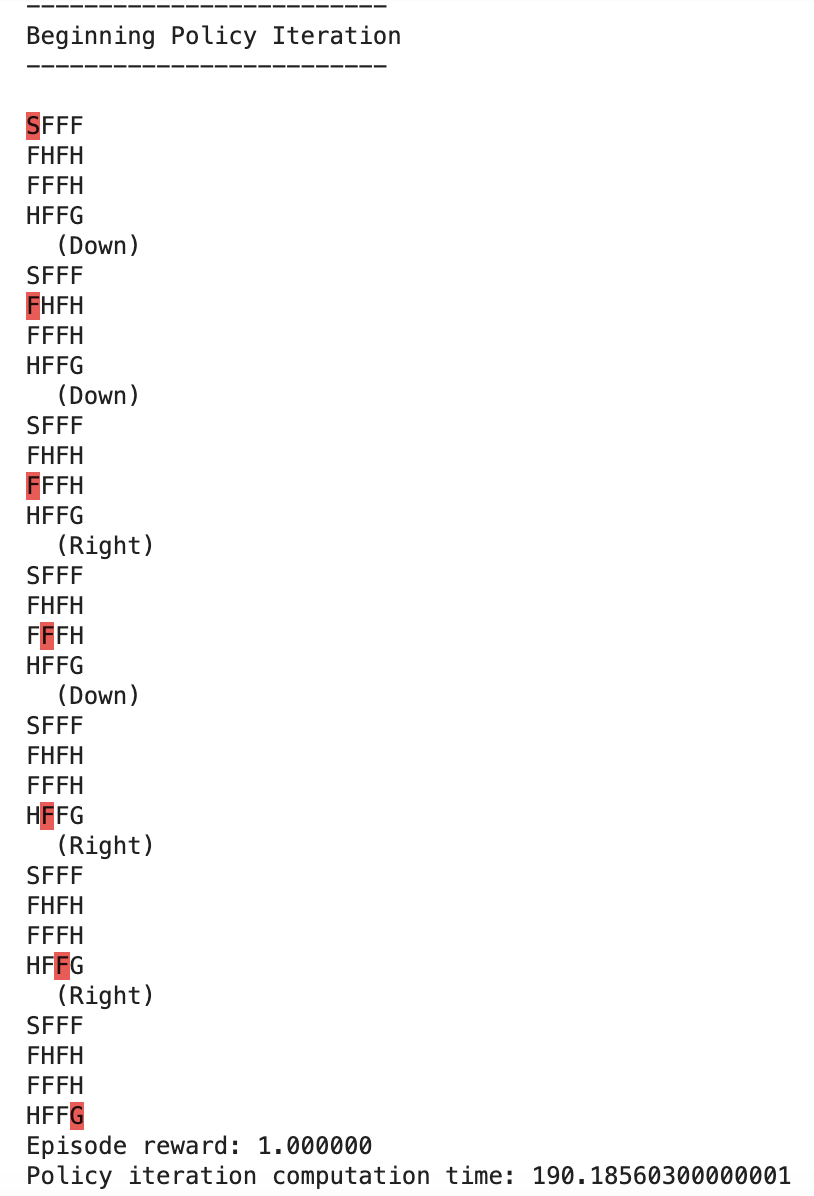
\includegraphics[width=7cm]{fig_pi_det.jpg} &
(b) & 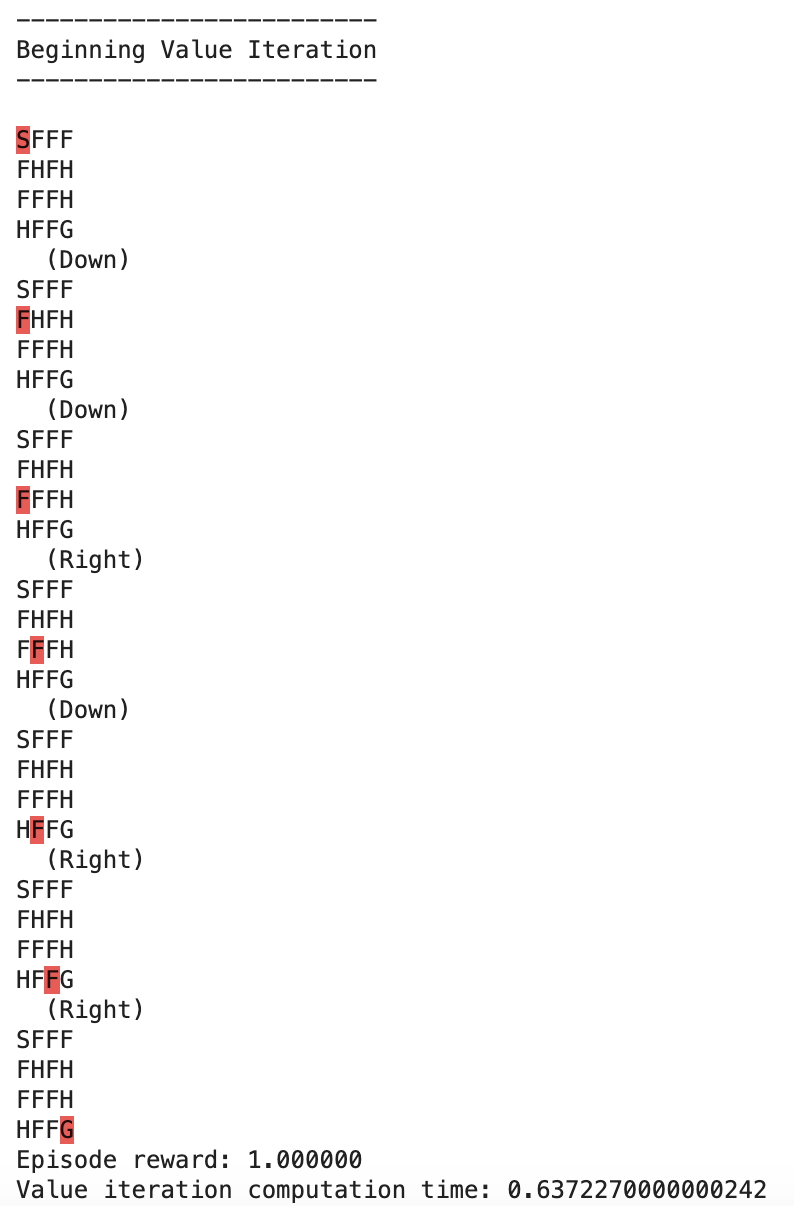
\includegraphics[width=7cm]{fig_vi_det.jpg} 
\end{tabular}
\captionof{figure}{Optimal policy found via (a) policy iteration and (b) value iteration. Below each table we present the computing time for comparison.}
\label{fig_op_det}
\end{center}


\subsection{}
We now re-run both value and policy iteration -based algorithm for the stochastic case (non-deterministic actions).

\begin{enumerate}
\item The value iteration: takes longer to converge and the optimal policy for stochastic case is different than in deterministic case (12 steps versus 7 steps).
\item The policy iteration: might not converge / needs much longer to converge. After the first run of 100 episodes it did not reach an optimal policy (ended up in a HOLE field instead of the target field). We re-ran it over 500 episodes for comparison and it did not converge either, hence we conclude it might either not converge at all, or do so asymptotically in which case computing the optimal policy is not computationally efficient.
\end{enumerate}

%\begin{center}
%\begin{tabular}{lclc}
%(a) & 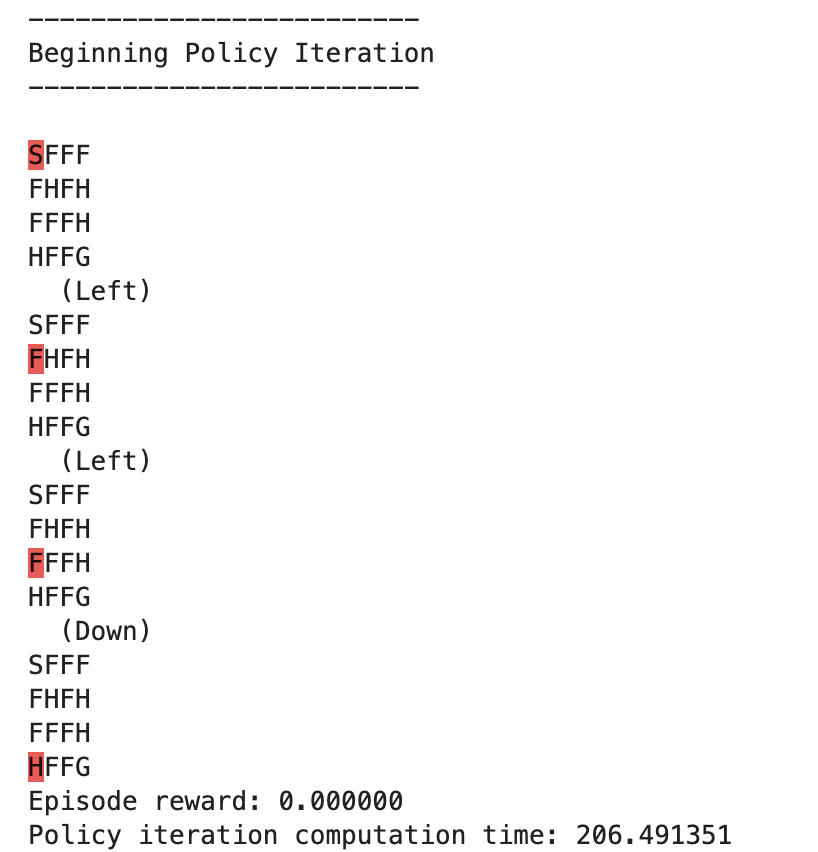
\includegraphics[width=7cm]{fig_pi_faulty.jpg} &
%(b) & \includegraphics[width=7cm]{fig_pi_sto.jpg} 
%\end{tabular}
%\captionof{figure}{Stochastic case, policy iteration:  (a) running over 100 episodes does not converge, (b) running over 200 episodes converges, albeit requires considerable computing time.}
%\label{fig_pi_sto}
%\end{center}

\section{}\label{question5}

We are concerned with a finite-horizon MDP, where agent is uncertain about the true dynamics of the MDP, and learns the system dynamics through exploration.

\cite{osband} develops posterior sampling for reinforcement learning (PSRL) which expands on the idea of Thompson sampling\cite{thompson}, and provides a bound on expected regret not based on optimism. The paper provides several experiments proving this approach to significantly outperform existing algorithms with similar regret bounds.

Majority of previous algorithms would adopt the OFU (\textit{optimism in the face of uncertainty}) rule. This means that the unknown parameters in the system are assigned maximum statistically possible value. This assumption is arbitrary. The agent is exploring poorly known policies, until it converges to optimal policy.

However, while useful in practice, there is no reason why OFU should be taken for granted. \cite{osband} develops an alternative approach, PSRL, where we optimize over MDP samples, taken at each iteration from the new, updated posterior distribution.

In summary, OFU explores the whole MDP by exploration of poorly understood policies. PSLR maximizes over sample each time, without prioritizing a particular policy. In this, PSLR is less biased in a way than OFU. It turns out that PSLR approach converges faster than OFU.

As a test, \cite{osband} applies PSRL to the River Swim problem, as well as several randomly generated MDPs.

As a further expansion, more testing could be conducted on examples were OFU is commonly used, to verify that PSRL is indeed a better approach. While providing an improved theoretical upper bound on expected regret, more experiments could better establish that this bound is indeed useful in practice (that the algorithm reaches close to the bound).

\begingroup
\let\clearpage\relax

\begin{thebibliography}{2}

\bibitem{osband}
Osband I., Russo D., Van Roy B., 
``(More) efficient reinforcement learning via posterior sampling'', \textit{Advances in Neural Information Processing Systems}, 2013, available at ArXiv: 1306.0940 (accessed 2020-03-28).

\bibitem{thompson}
Thomson, W.R.,
``On the likelihood that one unknown probability exceeds another in view of the evidence of two samples'', \textit{Biometrika}, 25(3/4):285-294, 1933
\end{thebibliography}
\endgroup
%\input{AccuracyLoss}

\end{document}